\chapter{Application}\label{D:application}

This chapter aims to develop the tasks introduced for the application layer in this project Gantt (see figure \ref{F:tpgp}).

\section{REST API}

As previously said, it's required to develop an API ready to be used over cloud environments in order to ease creating specific and new applications over the LMS framework, and thus to demonstrate the viability of this project prototype.

Nowadays, the common and widely used format for cloud services intercommunication is JSON, as it is also used for the TCP socket API of the LMS framework. Therefore, this API middleware is going to follow such premise.

A suitable technology to work with JSON formatted messages which is widely known for its good performance is Node.js (--REFERENCE--). Node.js is an open source, cross-platform runtime environment for server-side and networking applications. It provides an event-driven architecture and a non-blocking I/O API that optimizes application's throughput and scalability. This technology is commonly used for real-time web applications. 

Moreover, working with Node.js means avoiding serialization of the JSON messages by increasing services intercommunication performance (i.e.: less computational cost and less processing time). 

Then, the common Noje.js framework for developing web applications and REST APIs is Express.js (--REFERENCE--). It's the de facto standard server framework for Node.js. So, the middleware to develop is going to use its routing system, which refers to the definition of end points (URIs with HTTP request methods like GET, POST, PUT and DELETE) to an application and how it responds to client requests.

Following is the software structure proposal for developing the HTTP RESTfull API middleware, which is responsible to translate to the TCP socket API of the LMS framework:

\begin{figure}[!htb]
\begin{center}
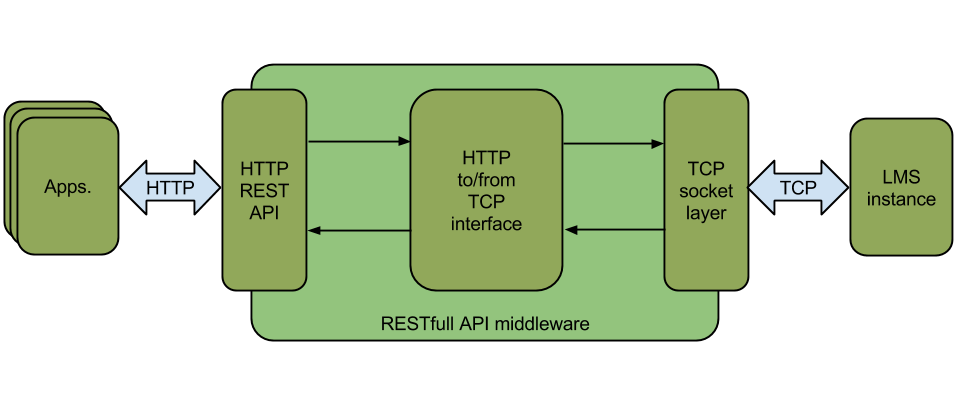
\includegraphics[width=1\textwidth]{./images/RESTAPI.png}
\caption{RESTfull API middleware architecture}
\label{F:restAPI}
\end{center}
\end{figure}

\begin{itemize}
\item HTTP REST API layer \hfill

This layer handles HTTP queries from external applications. It implements required routes to handle specific HTTP queries. First implementation will not implement multi LMS management but single. As shown in figure \ref{F:restAPI}.

\item Interface layer \hfill

This layer handles the body messages from the previous layer's HTTP queries and manipulates them in order to create an as much generic as possible API by adapting the messages to be sent through following layer.

\item TCP socket layer \hfill

This layer is the responsible to send and receive JSON formatted TCP socket messages between the LMS targeted instance.
\end{itemize}

As introduced in section {SOA:LMSframework} and deeply explained in ANNEX XX, there are two different management layers: the generic and the filter specific. So, by following this organization, the proposed API's structure is as shown next:

\begin{itemize}
\item Generic management queries
\begin{itemize}
\item Connect \hfill

Checks if an existing instance of LMS is running and sets the LMS port and LMS host to work with.
\begin{quote}
\begin{verbatim}
POST http://<host>:<port>/api/connect
JSON    {
            "port":<lms-port>,
            "host":"<lms-host>"
        }
\end{verbatim}
\end{quote}
\item Disconnect \hfill

Resets the running LMS instance and sets \verb|lms-port| and \verb|lms-host| to null in order to connect again to the same or any another LMS instance running.
\begin{quote}
\begin{verbatim}
GET http://<host>:<port>/api/disconnect
\end{verbatim}
\end{quote}
\item State \hfill

Gets the state object of the current LMS instance connected to (JSON object with the configured filters and paths).
\begin{quote}
\begin{verbatim}
GET http://<host>:<port>/api/state
\end{verbatim}
\end{quote}
\item Create a filter \hfill

Creates a filter (current types are: receiver, transmitter, demuxer, dasher, audioDecoder, audioEncoder, videoDecoder, videoResampler, videoEncoder, audioMixer, videoMixer) with an unique identifier.
\begin{quote}
\begin{verbatim}
POST http://<host>:<port>/api/createFilter
JSON    {
            "id": filterID,
            "type": "type"
        }
\end{verbatim}
\end{quote}        
\item Create a path of filters \hfill

Create a path of filters. A path can be a master path or an slave one, as shown:

\begin{itemize}

\item Master path
\begin{quote}
\begin{verbatim}
POST http://<host>:<port>/api/createPath
JSON    { 
            'id' : pathId, 
            'orgFilterId' : orgFilterId, 
            'dstFilterId' : dstFilterId, 
            'orgWriterId' : orgWriterId, 
            'dstReaderId' : dstReaderId, 
            'midFiltersIds' : [filterID1, filterID2,...] 
        }
\end{verbatim}
\end{quote}
\item Slave path of previous master path
\begin{quote}
\begin{verbatim}
POST http://<host>:<port>/api/createPath
JSON    { 
            'id' : pathId, 
            'orgFilterId' : filterID1, 
            'dstFilterId' : dstFilterId2, 
            'orgWriterId' : -1, 
            'dstReaderId' : dstReaderId2, 
            'midFiltersIds' : [filterID3, filterID4,...] 
        }  
\end{verbatim}
\end{quote}
\end{itemize}
\end{itemize}
\item Specific filter management queries        
\begin{itemize}
\item Configure an existing filter \hfill

Configures an existing filter (each filter has its own actions defined, check ANNEX XXX)
\begin{quote}
\begin{verbatim}
PUT http://<host>:<port>/api/filter/:filterID
JSON    [
            {
                "action":"the action",
                    "params":{
                        "param1":param1,
                        "param2":"param2",
                        "param3":"param3",
                        "param4":true
                }
            }
        ]
\end{verbatim}
\end{quote}

\end{itemize}
\end{itemize}

So, with previous API proposal, the whole TCP socket API becomes simplified.

Moreover, specific responses format to client has been proposed as shown:

\begin{itemize}
\item Success messages \hfill

It may be a string, bool, array or another object, depending on the request method

\begin{quote}
\begin{verbatim}
JSON    {
            "message": { the incoming message }
        }
\end{verbatim}
\end{quote}        
\item Error messages \hfill

\begin{quote}
\begin{verbatim}
JSON    {
            "error": "the error message"
        }
\end{verbatim}
\end{quote}
\end{itemize}

To point out that this API is not implementing persistence because the state (managed through 'State' method) is given by the LMS instance itself. The unique sign of persistence is regarding the LMS host and port which the middleware is connected to (managed through 'Connect' and 'Disconnect' methods). Higher levels of persistence should be implemented by external applications which implies specific scenarios and requirements (i.e.: specific persistence).

Finally, in order to know how this structure and the overall middleware is implemented check ANNEX XXX to see the code. Next chapters will demonstrate it too.

\section{Input network metrics}

As said in subsection \ref{B:appLayerCH2}, input network metrics are going to be implemented by carrying out methods re-implementations given by the Live555 library, which is the library implemented for managing network streams.  

\begin{figure}[!htb]
\begin{center}
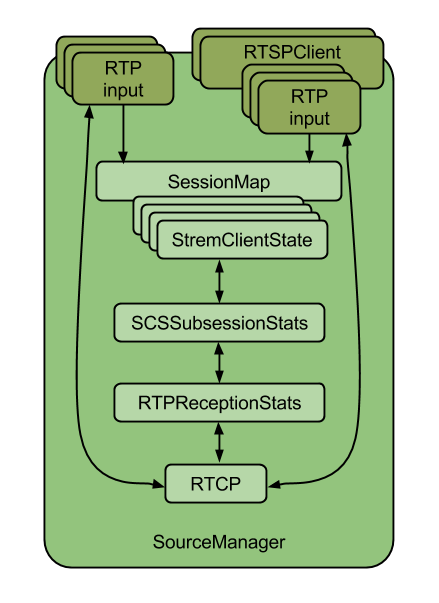
\includegraphics[width=0.45\textwidth]{./images/SourceManager.png}
\caption{Input network metrics structure}
\label{F:inms}
\end{center}
\end{figure}

By following the LiveMediaStreamer architecture structure, input network implementations are going to be implemented inside the 'liveMediaInput' structure. Concretely, a new class is implemented, called 'SCSSubsessionStats'. This class is managed by the 'StreamCleanState' class which is a class related to each stream 'Session' class managed by the 'SourceManager' class. This last class is a 'HeadFilter' class. Figure \ref{F:inms} shows the inter-class structure.

By initializing new RTP or RTSPClient sessions (i.e.: network inputs), a group of subessions is associated per each stream (i.e.: an RTP session has one subsession associated and the RTSPClient session has as many subsessions as accepted from the SDP that defines different RTP sessions).

When a new subsession is set, then, automatically, a new RTPReceiverStats class is initialized. This Live555 object implements RTCP stats measurement which are only required to be treated outside. This is done at SCSSubsessionState, which creates a new schedule to periodically measure and save current state (a default granularity of 1 second is set).

The implemented method that is called periodically is as shown:

\begin{quote}
\begin{verbatim}
void SCSSubsessionStats::
			periodicStatMeasurement(struct timeval const& timeNow) 
{
    unsigned secsDiff = timeNow.tv_sec - measurementEndTime.tv_sec;
    int usecsDiff = timeNow.tv_usec - measurementEndTime.tv_usec;
    double timeDiff = secsDiff + usecsDiff/1000000.0;
    measurementEndTime = timeNow;

    RTPReceptionStatsDB::Iterator statsIter(fSource->receptionStatsDB());

    RTPReceptionStats* stats = statsIter.next(True);
    if (stats != NULL) {
        double kBytesTotalNow = stats->totNumKBytesReceived();
        double kBytesDeltaNow = kBytesTotalNow - kBytesTotal;
        kBytesTotal = kBytesTotalNow;

        double kbpsNow = timeDiff == 0.0 ? 0.0 : 8*kBytesDeltaNow/timeDiff;
        if (kbpsNow < 0.0) kbpsNow = 0.0; // in case of roundoff error
        if (kbpsNow < kbitsPerSecondMin) kbitsPerSecondMin = kbpsNow;
        if (kbpsNow > kbitsPerSecondMax) kbitsPerSecondMax = kbpsNow;

        unsigned totReceivedNow = stats->totNumPacketsReceived();
        unsigned totExpectedNow = stats->totNumPacketsExpected();
        unsigned deltaReceivedNow = totReceivedNow - totNumPacketsReceived;
        unsigned deltaExpectedNow = totExpectedNow - totNumPacketsExpected;
        totNumPacketsReceived = totReceivedNow;
        totNumPacketsExpected = totExpectedNow;

        double lossFractionNow = deltaExpectedNow == 0 ? 0.0 : 1.0 -
        							 deltaReceivedNow/(double)deltaExpectedNow;

        if (lossFractionNow < packetLossFractionMin) {
            packetLossFractionMin = lossFractionNow;
        }
        if (lossFractionNow > packetLossFractionMax) {
            packetLossFractionMax = lossFractionNow;
        }

        minInterPacketGapUS = stats->minInterPacketGapUS();
        maxInterPacketGapUS = stats->maxInterPacketGapUS();
        totalGaps = stats->totalInterPacketGaps();
        jitter = stats->jitter();
    }
}
\end{verbatim}
\end{quote} 

Previous algorithm prepares the metrics that are going to be presented through the state when a new state query is received. For a more detailed insight of the overall implementation see ANEXX XX. Next is listed the metrics that are presented for new state queries:

\begin{itemize}
\item Bitrate: maximum, minimum and average in kbps.
\item Packet loss percentage: maximum, minimum and average.
\item Inter-packet gap: maximum, minimum and average in milliseconds.
\item Jitter: maximum, minimum and current inter-packet gap variation in microseconds.
\end{itemize}

Another metric that might be of interest is the time delay from the stream source but it is discarded due to not being offered from Live555 library. Moreover, to be implemented at SCSSubsessionStats class level has been discarded due to is computational cost and complexity to develop such requirement. But, to point out that it is not a high priority required metric due to take into account that this issue is out of LMS performance scope and if there are network performance problems they can be detected through other metrics already gathered.


\section{Output network metrics}

As said in subsection \ref{B:appLayerCH2}, output network metrics are going to be implemented by carrying out methods re-implementations given by the Live555 library, which is the library implemented for managing network streams.

This implementation has been much more difficult to be achieved due to not having control of the RTPSink class of the Live555 library in the sense of when it is deleted. Previous developments before the final version where based over the RTPSink re-implementation already done per each ServerMediaSubsession, which is also re-implemented. But the implementation was still losing the specific RTPSink instance of the subsession.

In order to go on the development an e-mail was sent to the Live555 developers mailing list, concretely to the head developer of the library, as shown next:

\begin{quote}
\begin{verbatim}
Sender: Gerard Castillo Lasheras <gerard.castillo@i2cat.net>
Receiver: LIVE555 Streaming Media - development & 
									use <live-devel@ns.live555.com> 
Hi Ross,

I'm implementing statistics on our software (liveMediaStreamer framework) 
and I'd like to have access to the RTPTransmissionStatsDB. But, I do not
see how to get the RTPSink object (which has the RTPTransmissionStatsDB 
and its stats).

Which should be the proper way to get the RTPSink object related to my
OnDemandServerMediaSubsession childs? I've seen that 
OnDemandServerMediaSubsession has a friend classe StreamState 
which has the RTPSink associated but, anyway, 
I'm not able to have access to it.

Thanks in advance,

Kind regards,
\end{verbatim}
\end{quote} 

The reply was concrete and helpful, as shown:
\begin{quote}
\begin{verbatim}
Sender: Ross Finlayson <finlayson@live555.com>
Receiver: LIVE555 Streaming Media - development & 
									use <live-devel@ns.live555.com> 
									
First of all, note that while a "OnDemandServerMediaSubsession" 
object refers to a track of streamable media, a “RTPSink" object 
refers to a receiving client (or possibly multiple clients if 
"reuseFirstSource" is True).  So there’s (in general) a 
one-to-many relationship between "OnDemandServerMediaSubsession" 
and "RTPSink".  Thus, it doesn’t make sense to talk about 
*the* RTPSink object for your "OnDemandServerMediaSubsession".

However…
There are at least two possible ways to get access to the 
"RTPSink" objects:

1/ Note the pure virtual function "createNewRTPSink()" that you 
have implemented in your "OnDemandServerMediaSubsession" subclass.  
You can use your implementation of this function to get access 
to the "RTPTransmissionStatsDB" for the new "RTPSink", after 
you’ve created it.
The drawback of this approach, though, is that you don’t know when 
the "RTPSink" object later gets deleted, so - if you’re not 
careful - you may end up holding a reference or pointer to a 
"RTPTransmissionStatsDB" that has been deleted.

2/ Define a subclass "myRTCPInstance" of the "RTCPInstance" 
class.  Then, in your "OnDemandServerMediaSubsession" subclass, 
reimplement the "createRTCP()" virtual function to create a 
"myRTCPInstance" object, rather than a "RTCPInstance" 
object.  Note that "createRTCP()" contains a "sink" 
parameter, pointing to a "RTPSink", from which you can 
get the "RTPTransmissionStatsDB".
The advantage of this approach over approach 1/ is that 
- by defining a subclass of "RTCPInstance", you can learn when 
the "RTPInstance" object gets deleted, and thus when the 
"RTPSink" object gets deleted.  (The "RTCPInstance" object 
always gets deleted immediately before the "RTPSink" 
object.)  Thus, you can use your "myRTCPInstance" destructor 
to figure out when the "RTPTransmissionStatsDB" should no 
longer be used.
									
\end{verbatim}
\end{quote} 

So, the best options, as suggested by Ross, was to re-implement the RTCPInstance class per each inherit class of the ServerMediaSession class, concretely the inherit classes of the QueueServerMediaSubsession class. 

\begin{figure}[!htb]
\begin{center}
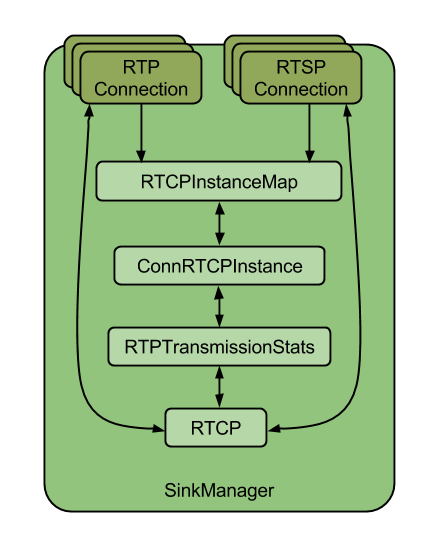
\includegraphics[width=0.45\textwidth]{./images/SinkManager.png}
\caption{Output network metrics structure}
\label{F:onms}
\end{center}
\end{figure}


\section{Frame delay metrics}

\section{Frame losses metrics}
